
\documentclass[13pt]{beamer}
% \ProvidesPackage{preambles}
% \ProvidesPackage{preamblesnotes}
\usepackage{fontsize}
\usepackage{amsmath,amssymb,amsthm}
\usepackage{graphicx} % Required for inserting images
\usepackage{xeCJK}
\setCJKmainfont[AutoFakeBold=true]{TW-Sung}
% \setCJKmainfont[AutoFakeBold=true]{LiSong Pro}
\usepackage{tabto}
\usepackage{parskip}  % No-indent
\usepackage{enumitem} % change enumerate behaviours
\usepackage{lipsum} %
\usepackage{color}
\usepackage{siunitx}
\usepackage{newclude} %make include only not clearpage
\usepackage{multicol}
\usepackage{adjustbox}
\usepackage{multirow}
\usepackage{soul}
\usepackage{tasks}
\usepackage{tcolorbox}
\usepackage[version=4]{mhchem}
\usepackage{tabularray}
\usepackage{probsoln}
% turning \beginfigure


\newcommand{\here}[1]{
    {\par\centering #1
            \par}
}

\newcommand{\bshere}[1]{
    {\bigskip\par\centering #1
            \par\bigskip}
}

\NumTabs{5}
\newcommand{\dtab}{ \tab\tab }
\newcommand{\om}[1]{ \qty{#1}{\ohm}}
% \usepackage{minipages}

% \setlength{\tabcolsep}{20pt}
\renewcommand{\arraystretch}{1.5}

\def\sd {(\arabic*)}
% \marksnotpoints
% \marginpointname{ 分\points}
% \renewcommand{\thequestion}{\Roman{question}}
\pointsinrightmargin
\pointpoints{mark}{marks}
\pointname{ \points}

% \setcounter{totalnumber}{30}% lots of here floats

\def\a{One two \stepcounter{enumi}\roman{enumi} three four five six. }
\def\b{\a\a  red \stepcounter{enumi}\roman{enumi} red green yellow 
random longer typesetting expressions that might invoke hyphenation. }
\def\c{\a\b\a\a\b\b\a}

\def\f#1{\begin{figure}[hp]\centering\rule{2cm}{1cm}\par\caption{ff: #1}\end{figure}}
\def\t#1{\begin{table}[hp]\centering\caption{tt: #1}\par\bigskip\begin{tabular}{cc}1&2\\33&44\\555&666\end{tabular}\end{table}}

\makeatletter
\def\flushhere{\par{%
 \let\s@deferlist\@deferlist
 \let\@currbox\relax
\@next\@currbox\@deferlist{%
  \ifodd\count\@currbox
\typeout{Trying \meaning\@currbox (\number\@currbox/\the\count\@currbox),
        adding to \meaning\@currlist}%
    \@cons\@currlist\@currbox
\typeout{added: to \meaning\@currlist}%
\typeout{deferlist was \s@deferlist, now \@deferlist}%
\let\s@@deferlist\@deferlist\@empty
\global\let\@deferlist\@empty
    \@floatpenalty -\@Miii
      \penalty -\@Miv
      \@tempdima\prevdepth
      \vbox{}%
      \prevdepth\@tempdima
      \penalty\@floatpenalty
       \@@par
   \ifx\@deferlist\@empty
\typeout{float placed here}%
\global\let\@deferlist\s@@deferlist
   \flushhere
\else
\typeout{float not placed here}%
\global\let\@deferlist\s@deferlist
\fi
    \else
\typeout{not h}%
    \global\let\@deferlist\s@deferlist
    \fi
   }%
  {%
\typeout{no pending float}%
}\par}}

\makeatother

\newcommand{\oneTwo}[5][example]{
    \begin{#1}
    \par #2\ \begin{enumerate}[label=\sd ]
        \item #3
        \item #4
        \item #5
    \end{enumerate}

    \end{#1}
}
\newcommand{\shc}[1]{
    \qty[mode = text]{#1}{J.kg^{-1}.\degreeCelsius^{-1}}
}
\newcommand{\hc}[1]{
    \qty[mode = text]{#1}{J.\degreeCelsius^{-1}}
}
\newcommand{\oc}[1]{
    \qty{#1}{\degreeCelsius}
}

\newcommand{\dg}[1]{$#1^{\circ}$}

\newcommand{\slh}[1]{\qty{#1}{J.kg^{-1}}}

\newcommand{\vel}[1]{
    \qty{#1}{m.s^{-1}}
}
\newcommand{\kmh}[1]{
    \qty{#1}{km.h^{-1}}
}
\newcommand{\acc}[1]{
    \qty{#1}{m.s^{-2}}
}
% \newcounter{mchoice}
\renewcommand{\themchoice}{\Alph{mchoice}}
\newcommand\mchoicelabel{\themchoice.}
\newcounter{schoice}
\newcommand\schoicelabel{(\theschoice)}

\newenvironment{mchoices}%
  {\list{\mchoicelabel}%
     {\usecounter{mchoice}
       \settowidth{\leftmargin}{W.\hskip\labelsep\hskip 2.5em}%
       \def\choice{%
         \item
       } % choice
       \labelwidth\leftmargin\advance\labelwidth-\labelsep
       \topsep=15pt
       \partopsep=0pt
     }%
  }%
  {\endlist}
\newenvironment{schoices}
{\list{\schoicelabel}%
     {\usecounter{schoice}
       \settowidth{\leftmargin}{W.\hskip\labelsep\hskip 1.5em}%
       \def\choice{%
         \item
       } % choice
       \labelwidth\leftmargin\advance\labelwidth-\labelsep
       \topsep=15pt
       \partopsep=0pt
     }%
  }%
  {\endlist}

  \newcommand{\topalign}[1]{
  \adjustbox{valign=t}{
    #1
}
  }


\pagestyle{headandfoot}
% \runningheadrule
% \firstpageheader{熱學第二課}{熱和內能}{2024年9月2日}
% \runningheader{熱學第二課}
% {熱和內能 Heat and Internal Energy, Page \thepage\ of \numpages}
% {2024年9月2日}
% \lhead{\ifcontinuation{Question \ContinuedQuestion\ continues\ldots}{}}
% \chead{熱和內能 Heat and Internal Energy}
\rhead{Page \thepage\ of \numpages}


% tasks package
\settasks{label=\Alph*.,item-indent=5.5em, before-skip=1.8em, after-item-skip=.35em,after-skip = 1.2em,label-offset=2.5em}
\NewTasksEnvironment[item-format={\topalign}, label=\Alph*., before-skip=1.5em]{mcimg}(2)
\NewTasksEnvironment[label=(\arabic*)]{statements}


%  an additional 0.5 inch of blank space inserted between questions
\renewcommand{\questionshook}{\setlength{\itemsep}{0.2in}}

\NumTabs{5}
\setlength\linefillheight{.5in}
\setlength\dottedlinefillheight{.5in}

% \includeonly{mc,lq} % include which file ###################################

\newcommand{\setup}[2]{

    {\LARGE\textbf{#1}}\hfill\makebox[0.25\textwidth]{姓名:\enspace\hrulefill}

    {\noindent\par{\LARGE\textbf{#2}}
        % \hfill\makebox[0.24\textwidth]{學號:\enspace\hrulefill}
        \vspace{10mm}}
}

\newcommand{\newprob}[3]{

    \begin{defproblem}{#1}%
        #2
        \begin{onlysolution}%
            #3
        \end{onlysolution}%
    \end{defproblem}
}

\newcommand{\ansdisplay}{
    \showanswers\printanswers
}


\newcommand{\dlines}[1]{
    \ifprintanswers

    \else
        \fillwithdottedlines{\stretch{#1}}
    \fi
}


\newcommand{\ddlines}[1]{
    \ifprintanswers

    \else
        \fillwithdottedlines{#1in}
    \fi
}

\newcommand{\mcq}[1]{
    \filbreak\question
    \useproblem{#1}
}

\newcommand{\topalign}[1]{
    \adjustbox{valign=t}{
        #1
    }}
\newcommand{\topalignc}[1]{
    \adjustbox{valign=t, center}{
        #1
    }}

\newcommand{\zh}[1]{\hfill (#1 marks)}
\newcommand{\zzh}[1]{\hfill (#1 分)}

\renewcommand{\thesubsubpart}{\arabic{question}}
\renewcommand{\subpartlabel}{(\thesubpart)}
\renewcommand{\subsubpartlabel}{(\thesubsubpart)}

\newcommand{\ans}[1]{\ifprintanswers
        \textbf{Ans:} {\color{red}#1}
    \fi}
\newenvironment{ansblock}{\ifprintanswers
        }{\fi}

\renewcommand{\labelenumi}{(\alph{enumi})}
\renewcommand{\labelenumii}{(\roman{enumii})}
\graphicspath{{../../assets}}

%Information to be included in the title page:
\title{第五課}
\author{動量 I Momentum I}
\institute{周末班}
\date{}

\begin{document}
\frame{\titlepage}

% \begin{frame}{動量是什麼?What is momentum}

% \end{frame}

\begin{frame}{動量Momentum}
    \begin{itemize}
        \item 質量和速度的乘積\\The product of mass and velocity
    \end{itemize}
    \begin{alertblock}
        {動量Momentum $\vec{p}$}
        \begin{equation}
            \vec{p}=m\vec{v}
        \end{equation}
    \end{alertblock}
    \begin{itemize}
        \item 動量是向量\\Momentum is vector
        \item 單位Unit: [\unit{kg.m.s^{-1}}] or [\unit{N.s}]
    \end{itemize}
\end{frame}

\begin{frame}{動量改變Momentum change}
    動量的改變 $=$ 最終動量 $–$ 起始動量\\Momentum change $=$ final momentum $-$ initial momentum
    \begin{exampleblock}
        {動量的改變Momentum change $\Delta \vec{p}$}
        \begin{equation}
            \Delta\vec{p}=m\vec{v}-m\vec{u}
        \end{equation}
    \end{exampleblock}
\end{frame}

\begin{frame}{動量改變Momentum change}
    \begin{itemize}
        \item 要注意動量本身是有方向的:\\Note that momentum itself has direction:
        \item 例如,取向右的方向為正:\\For example, take right direction as positive:
    \end{itemize}
    {\par\centering
    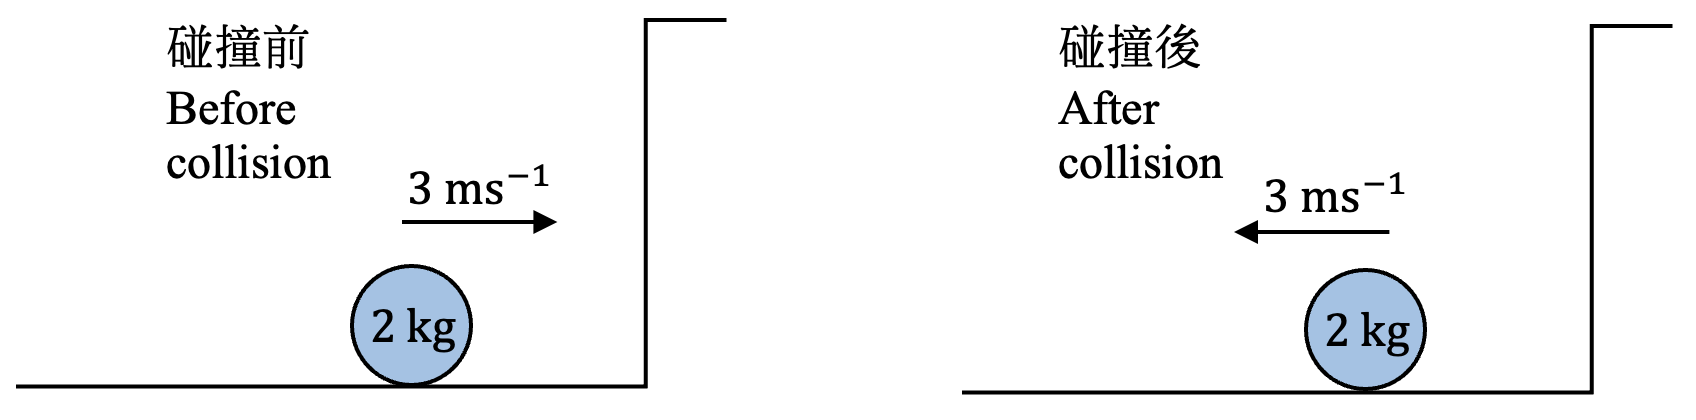
\includegraphics[width=0.66\textwidth]{assets/e26d5e2e.png}
    \par}
    \begin{itemize}
        \item[]\begin{itemize}
                  \item 動量的改變 Momentum change
                  \item[] $\Delta p=mv-mu=(2)(-3)-(2)(3)=\qty{-12}{kg.m.s^{-1}}$
                  \item 動量的改變量值 Magnitude of momentum change $=$ \qty{12}{kg.m.s^{-1}}
              \end{itemize}
    \end{itemize}
\end{frame}

\begin{frame}{動量改變Momentum change}
    例 For example:
    {\par\centering
    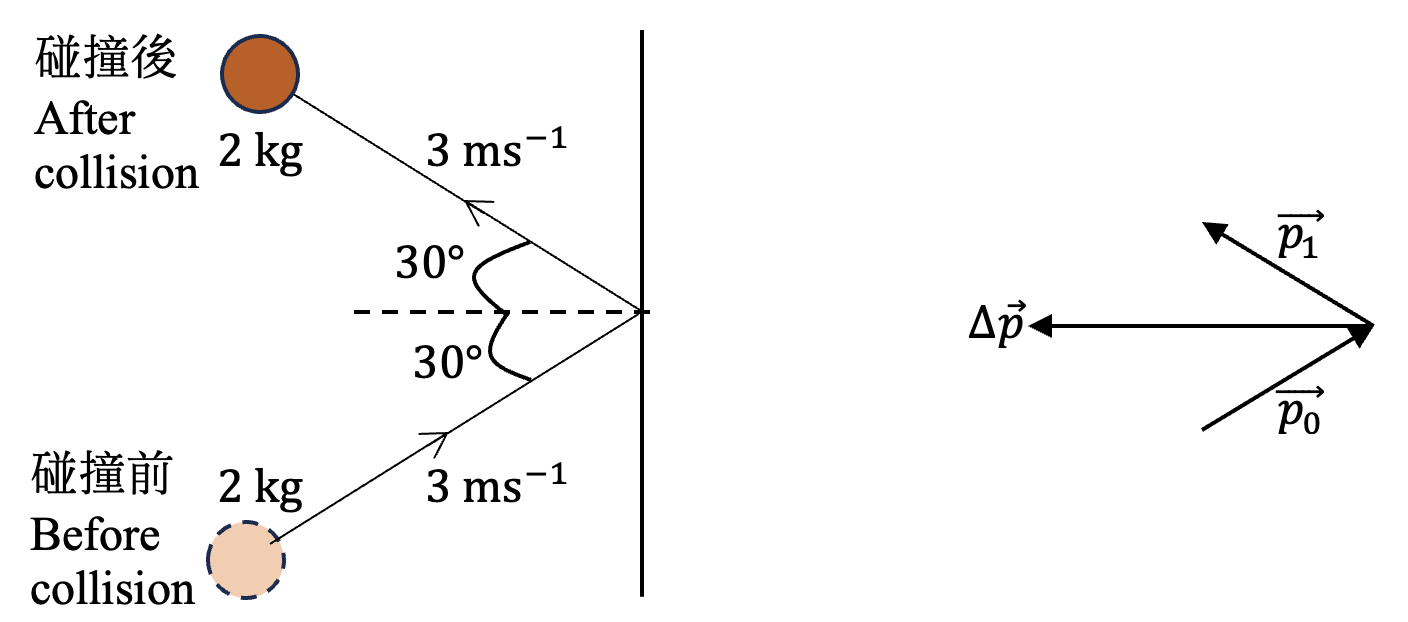
\includegraphics[width=0.66\textwidth]{assets/4c46ae9d.png}
    \par}
    \begin{itemize}
        \item 取向右的方向為正:\\For example, take right direction as positive:
        \item 動量的改變只有水平的方向:\\ There is only momentum change in the horizontal direction:
        \item[] $\Delta p=m\vec{v}-m\vec{u}=(2)(-3)\cos 30^\circ-(2)(3)\cos 30^\circ=\qty{-10.4}{kg.m.s^{-1}}$
    \end{itemize}
\end{frame}

\begin{frame}{牛頓第二定律Newton's second law}
    \begin{itemize}
        \item 一個系統在外力作用下,必定會有動量變化。\\When a system is under external force, there will be a change of momentum.
              \begin{itemize}
                  \item [] \textbf{淨力Net force} $F_{net}=ma=\dfrac{m\Delta v}{\Delta t}=\dfrac{\Delta p}{\Delta t}$
              \end{itemize}
    \end{itemize}
    \begin{alertblock}
        {牛頓第二定律的動量版本Newton's second law in terms of momentum}
        \begin{equation}
            F_{net}=\frac{\Delta p}{\Delta t}=\frac{mv-mu}{\Delta t}
        \end{equation}
    \end{alertblock}
\end{frame}

\begin{frame}{牛頓第二定律Newton's second law}
    \begin{itemize}
        \item[] \fbox{$F=\dfrac{mu-mu}{t}$}
    \end{itemize}
    {\par\centering
    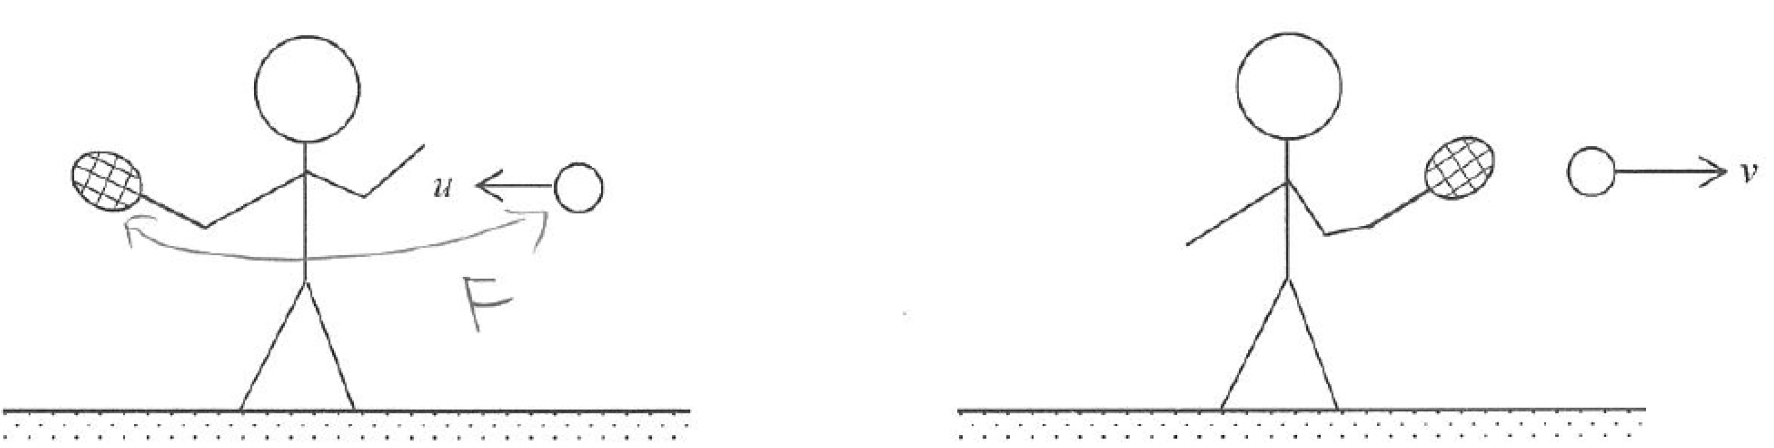
\includegraphics[width=0.66\textwidth]{assets/bc5b866b.png}
    \par}
\end{frame}


\begin{frame}{牛頓第二定律Newton's second law}
    e.g.
        {\par\centering
            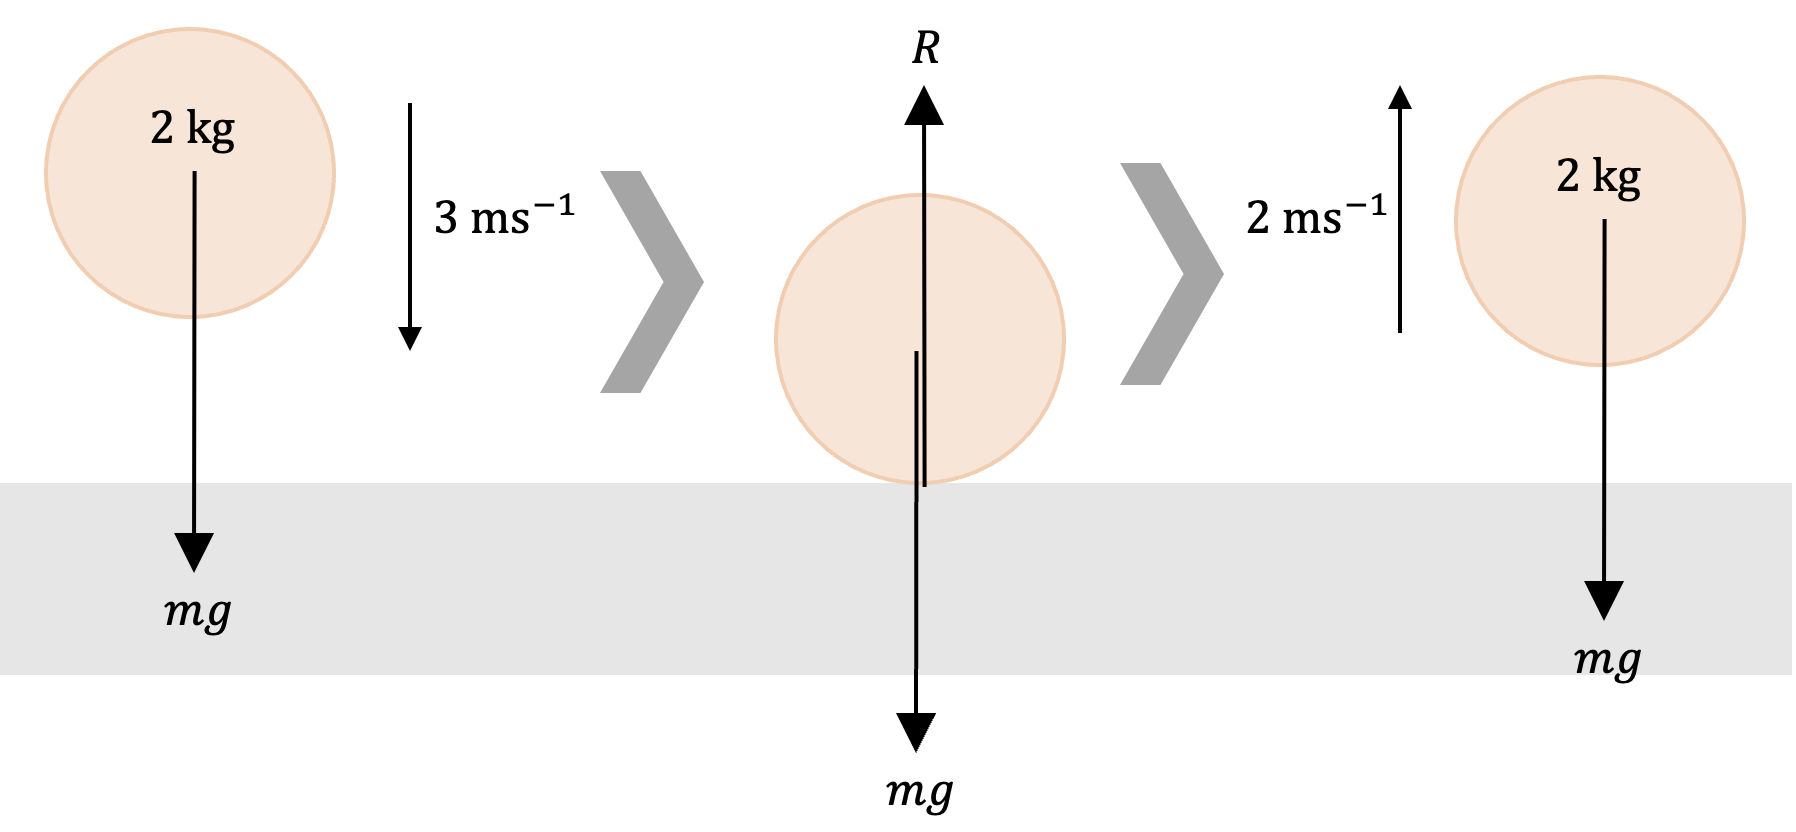
\includegraphics[width=.8\textwidth]{assets/16fb42f7.png}
            \par}



\end{frame}
\begin{frame}{牛頓第二定律Newton's second law}
    己知碰撞時間是 \qty{0.1}{s},求碰撞期間地面施加的力。\\Given collision time is \qty{0.1}{s}, find force exerted by the ground  during collision.\medskip
    \begin{columns}
        \column{.5\textwidth}
        \begin{itemize}
            \setlength{\itemsep}{0.6em}
            \item 取向上為正,\\Take upward direction as positive.
            \item []$F_{net}=R-mg = \dfrac{mv-mu}{t}$
            \item []$R-(2)(9.81)=\dfrac{2(2)-2(-3)}{0.1}$
            \item [] $R=\qty{119.62}{N}$
        \end{itemize}
        \column{.5\textwidth}
        \begin{itemize}
            \setlength{\itemsep}{0.6em}
            \item 取向下為正,\\Take downward direction as positive.
            \item []$F_{net}=mg-R = \dfrac{mv-mu}{t}$
            \item []$(2)(9.81)-R=\dfrac{2(-2)-2(3)}{0.1}$
            \item [] $R=\qty{119.62}{N}$
        \end{itemize}

    \end{columns}
\end{frame}


\begin{frame}{連續流動的物體Continuous flowing objects}
    \par
    {\par\centering
        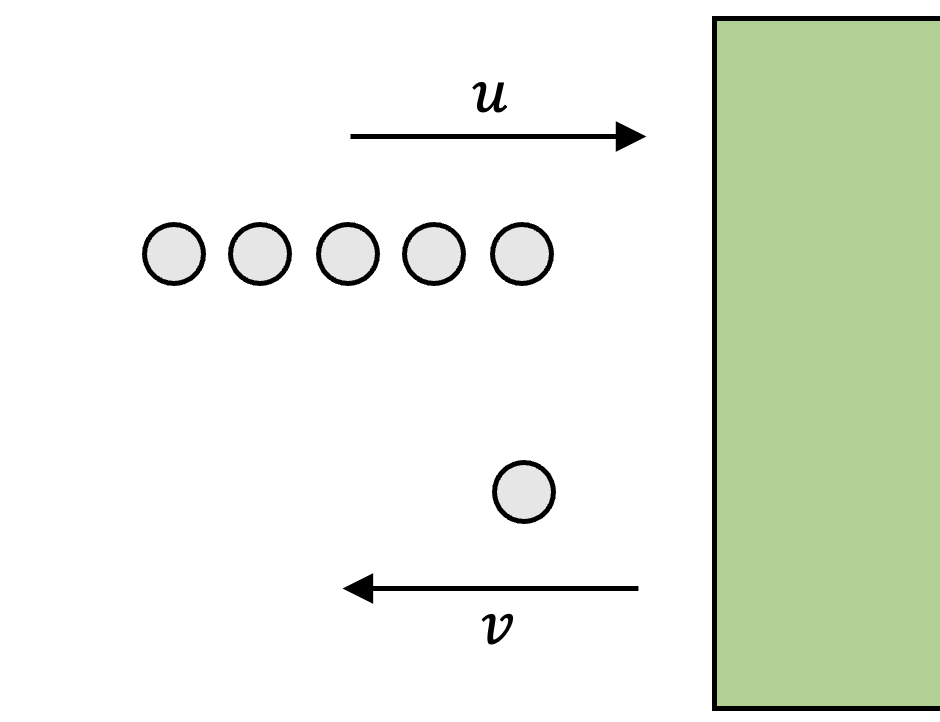
\includegraphics[width=.4\textwidth]{assets/9bad99da.png}
        \par}
    \begin{itemize}
        \item \fbox{$F=\dfrac{m}{t}(v-u)$}
        \item 其中 $\dfrac{m}{t}$是質量的改變/流動速率。
        \item [] And $\dfrac{m}{t}$ means rate of change of mass/rate of flow of mass.
    \end{itemize}
\end{frame}

\begin{eg}
    \par{\par\centering
        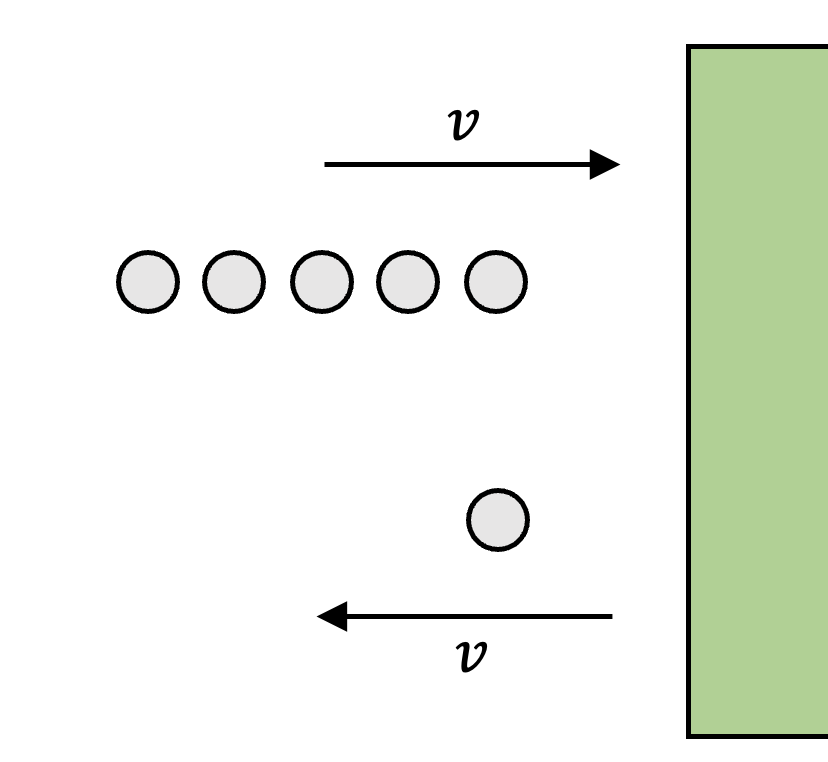
\includegraphics[width=.4\textwidth]{assets/75a1ea9d.png}
        \par}
    子彈以每秒 $n$ 個的發射速率射擊牆壁,每個子彈的質量為 $m$,並以水平速度 $v$ 撞擊牆壁後以相同的水平速度 $v$ 彈回。以下哪個陳述正確?\\Bullets are fired at a rate of $n$ per second at a wall, with each bullet having a mass of $m$ and impacting the wall with a horizontal velocity of $v$ before rebounding with the same horizontal velocity $v$. Which of the following statements is correct?

\end{eg}

\begin{eg}
    \begin{tasks}
        \task [(1)] 子彈的總動量變化是$0$。\\Total change of momentum of bullets is $0$.
        \task [(2)] 子彈每秒的總動量變化是2mnv。\\Total change of momentum of bullets per second is $2mnv$.
        \task [(3)] 牆壁所受的平均力是2mnv。\\Average force experienced by the wall is $2mnv$.
    \end{tasks}
\end{eg}

\begin{frame}{動量守恆定律Conservation of momentum}
    \par{\par\centering
        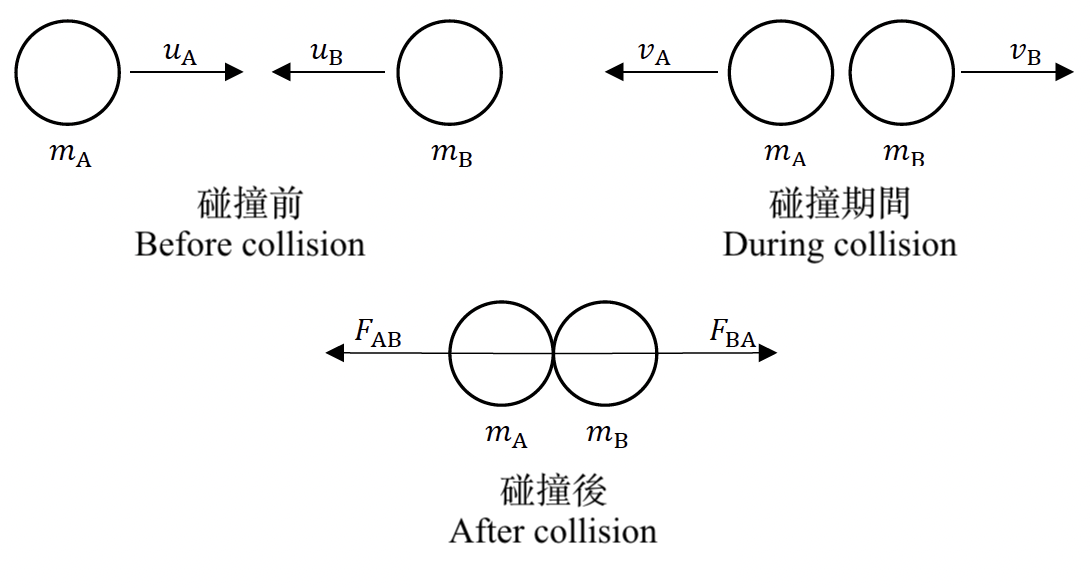
\includegraphics[width=0.8\textwidth]{assets/02c41700.png}
        \par}
\end{frame}
\begin{frame}{動量守恆定律Conservation of momentum}
    \begin{itemize}
        \item 根據牛頓第三定律,\\By Newton's third law,
        \item []$F_{AB}=-F_{BA}$
        \item 若沒有外力施於物體,\\If there is no external force acting on the object,
        \item []$\dfrac{m_A(v_A-u_A)}{t}=-\dfrac{m_B(v_B-u_B)}{t}$
        \item 透過移項可得\\Arranging the terms we can get
        \item []$m_Au_A+m_Bu_B=m_Av_A+m_Bv_B$
    \end{itemize}
\end{frame}
\begin{frame}{動量守恆定律Conservation of momentum}

    \begin{alertblock}
        {動量守恆定律Conservation of momentum}
        \begin{equation}
            m_Au_A+m_Bu_B=m_Av_A+m_Bv_B
        \end{equation}
    \end{alertblock}
    \begin{itemize}
        \item 換言之,一個系統的起始動量總和,等於最終動量總和。\\In other words, the inital sum of momentum in a system, equals final sum of momentum.
        \item 同樣要注意 $u$ 和 $v$ 也是可以是正或負號。正負號取決於哪個方向取作正。\\Again, note that $u$ and $v$ could be positive or negative, depending on which direction we take as positive.
    \end{itemize}
\end{frame}

\begin{eg}
    質量為 \qty{1000}{kg} 的汽車 P 以 \vel{20} 的速度向前行駛,並與質量為 \qty{1500}{kg} 的汽車 Q 發生正面碰撞。在碰撞前,汽車 Q 以 \vel{10} 的速度朝相反方向行駛。如果兩輛汽車在碰撞後黏在一起,請找出碰撞後它們的共同速度。\\A car P with a mass of \qty{1000}{kg} is moving forward at a velocity of \vel{20} and collides head-on with a car Q with a mass of \qty{1500}{kg}. Prior to the collision, car Q is traveling in the opposite direction with a velocity of \vel{10}. If the two cars stick together after the collision, find their common velocity after the collision.
\end{eg}

% \begin{eg}
%     一枝火箭最初在太空中靜止不動,火箭接著發生爆炸並分裂為 兩部分。該兩部分沿相反方向運動。若後部分的質量較前部分 的為大,下列哪一項敍述是正確的?
% \end{eg}

\begin{frame}{力和動量的關係線圖Relation graphs between force and momentum}
    \par{\par\centering
        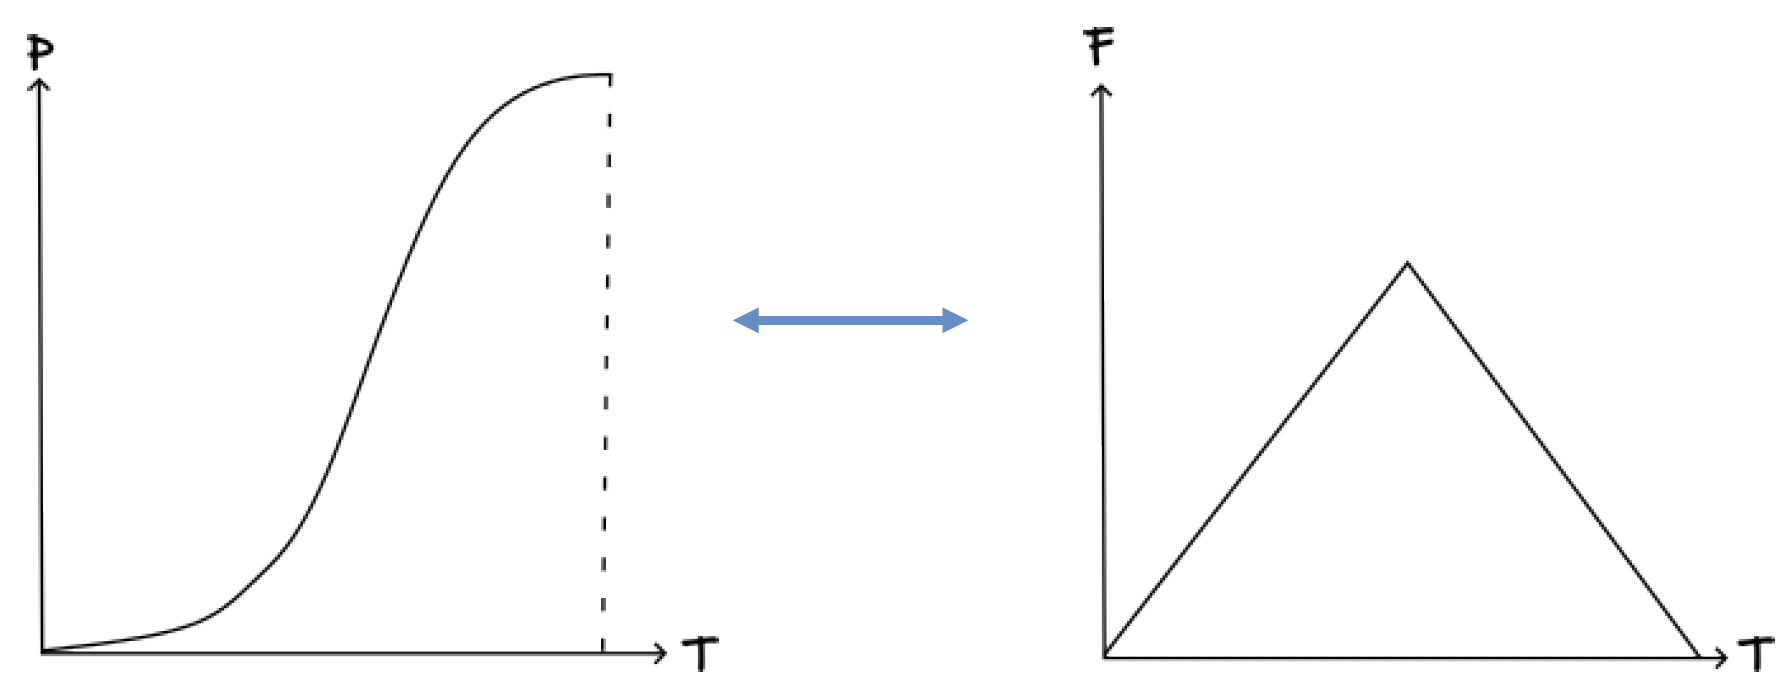
\includegraphics[width=\textwidth]{assets/a8d214ae.png}
        \par}
    \bigskip
    \begin{itemize}
        \item []$\because F=\dfrac{\Delta p}{\Delta t}$,\hspace{1em}$p-t$線圖的斜率$=$$F-t$線圖的值。\\Slope of $p-t$ graphs $=$ value of $F-t$ graphs.
    \end{itemize}
\end{frame}





\begin{frame}{力和動量的關係線圖Relation graphs between force and momentum}
    \par{\par\centering
        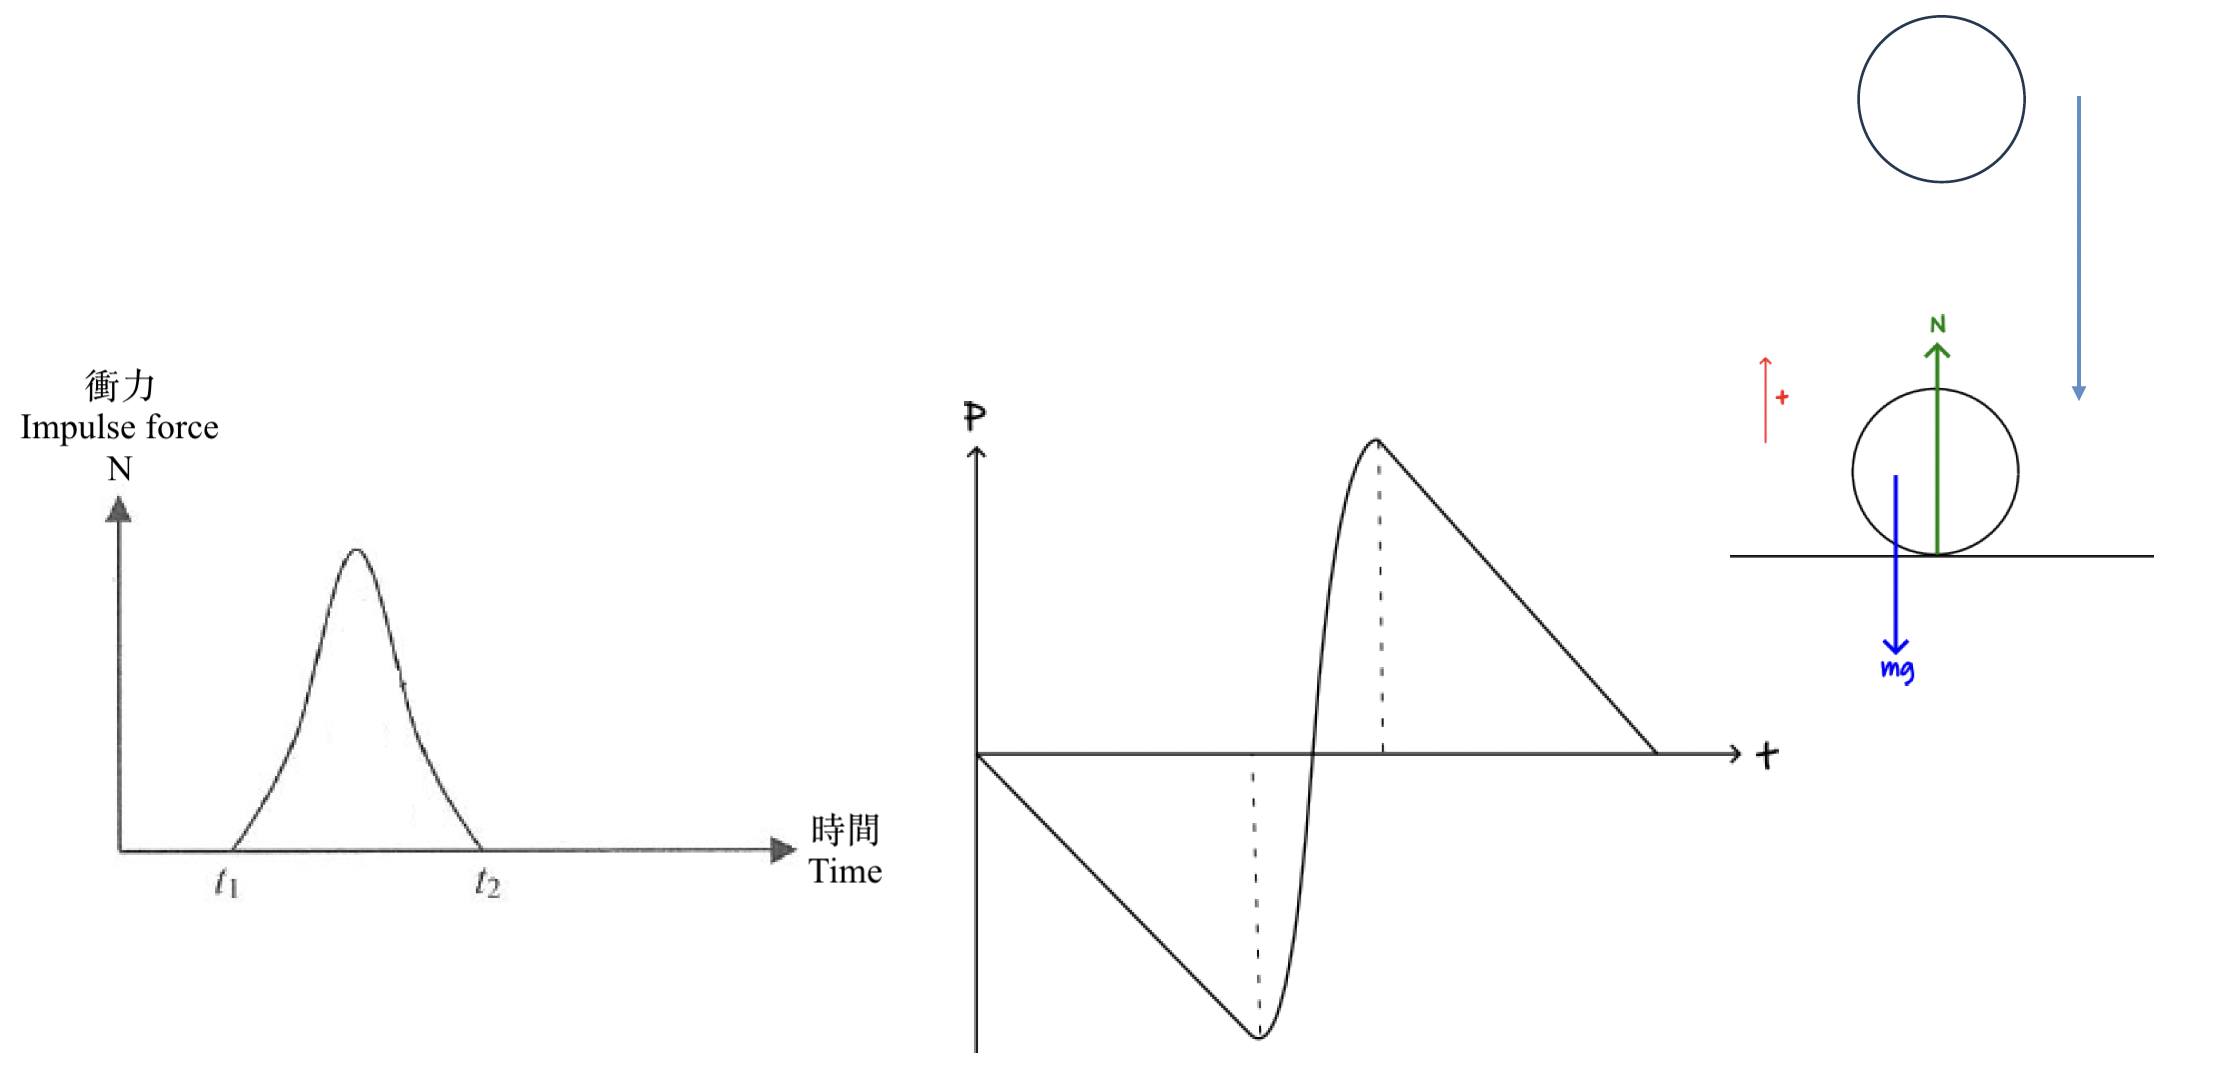
\includegraphics[width=\textwidth]{assets/f231d810.png}
        \par}
\end{frame}


\begin{frame}{力和動量的關係線圖Relation graphs between force and momentum}
    \par{\par\centering
        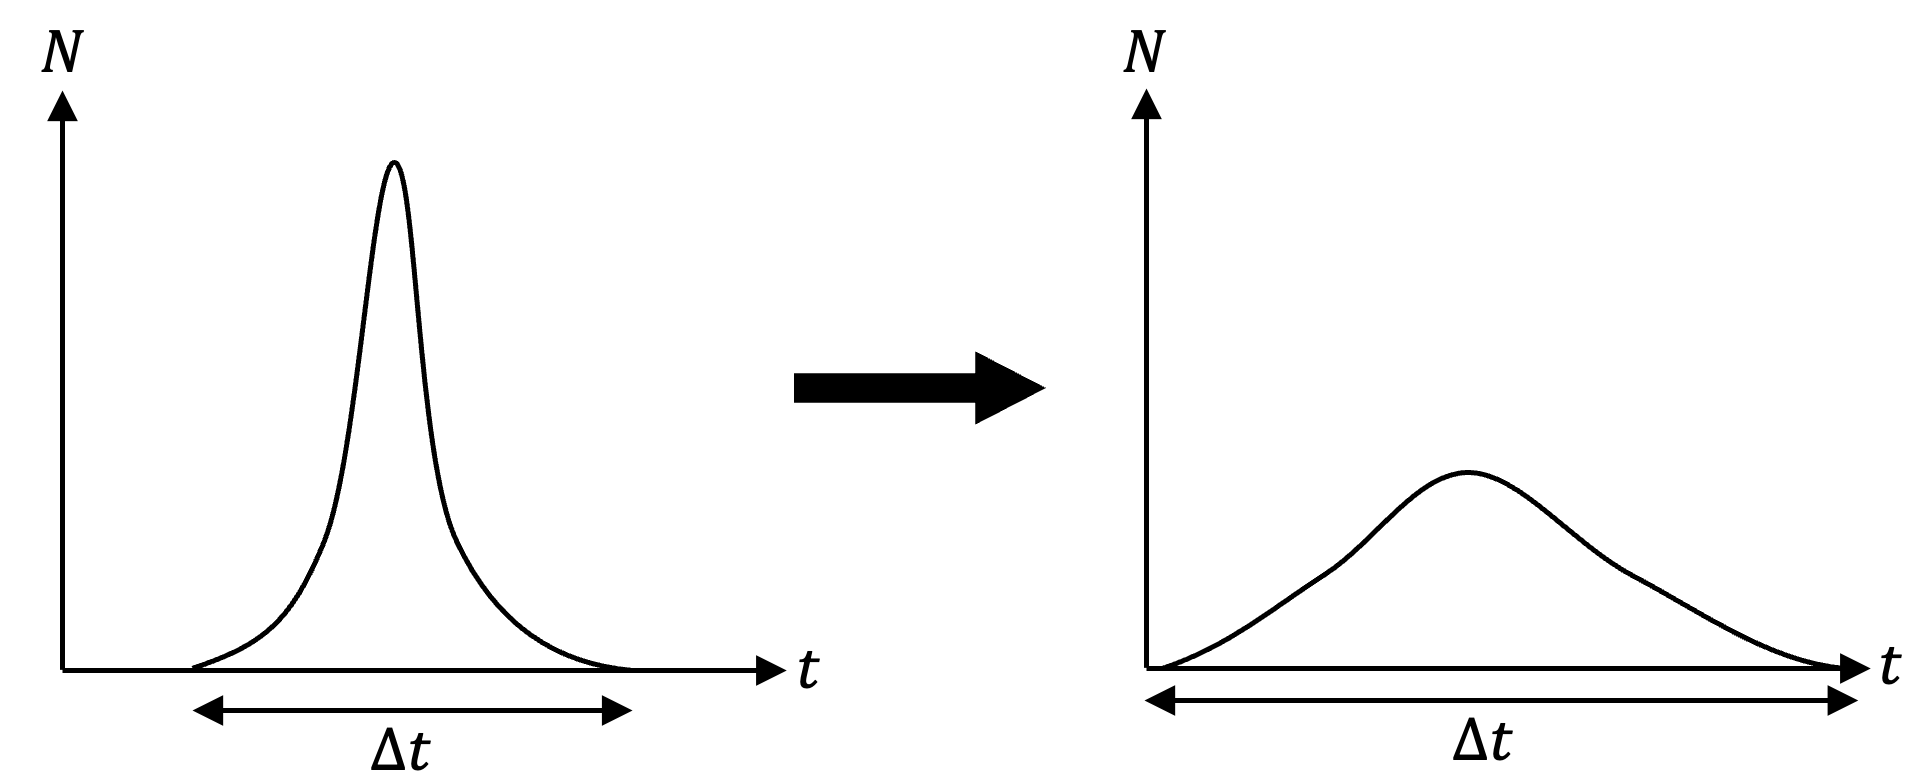
\includegraphics[width=.8\textwidth]{assets/76cc933c.png}
        \par}\bigskip
    \begin{itemize}
        \item 增加撞擊的持續時間$\Delta t$, 可以減少受到的平均衝力 $N$。\\When collision time $\Delta t$ is increased, the average impulse force can be reduced.
    \end{itemize}
\end{frame}

\begin{frame}{力和動量的關係線圖Relation graphs between force and momentum}
    \par{\par\centering
        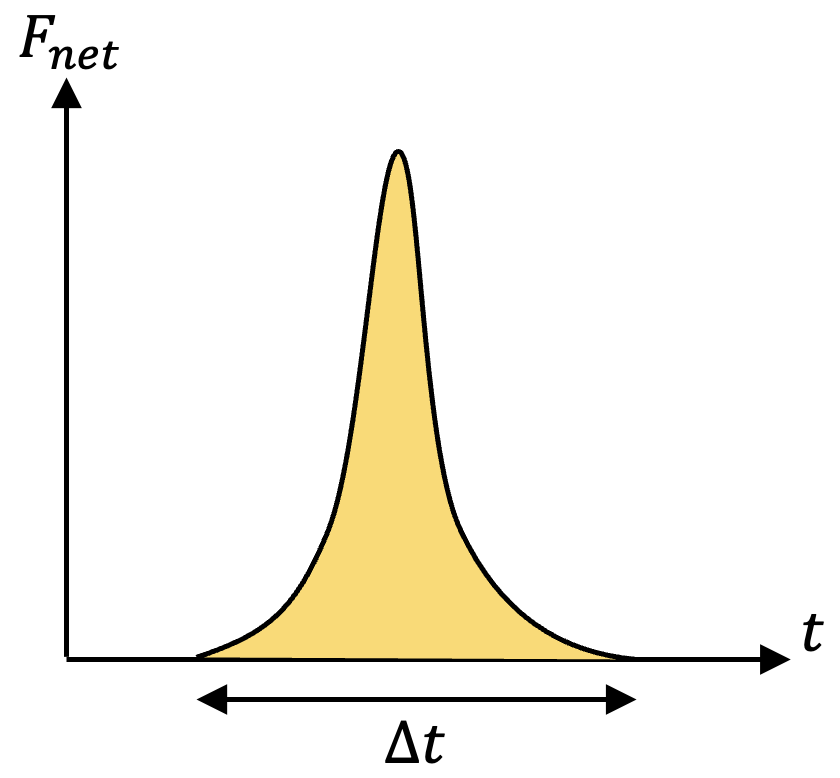
\includegraphics[width=.3\textwidth]{assets/99524ca7.png}
        \par}
    \begin{alertblock}
        {衝量定義Difinition of impulse}
        \begin{itemize}
            \item 衝量Impulse $=mv-mu$
            \item []$=F_{net}-t$ 線圖下的\textbf{面積}\\$=$ \textbf{Area} under $F_{net}-t$ graphs.
        \end{itemize}
    \end{alertblock}

\end{frame}

\begin{frame}{}
    一顆蛋如果從高處掉落並落在硬表面上,很可能會破裂。然而,如果蛋從相同的高度掉落,但落在軟墊上,它可能不會破裂。這是因為使用軟墊時,\\An egg will probably break if it is released at a height and lands on a hard surface. However, the egg may not break if it is released at the same height but lands on a soft cushion. it is because, when the cushion is used,
    \begin{itemize}
        \item[A.] 蛋在撞擊前的動量變小。\\the momentum of the egg just before impact becomes smaller.
        \item[B.] 蛋撞到軟墊後反彈。\\the egg rebounds after hitting the cushion.
        \item[C.] 蛋在撞擊期間的動量變化率變小。\\the rate of change of momentum of the egg becomes smaller during the impact.
        \item[D.] 軟墊對蛋的作用力比蛋對軟墊的作用力小。\\the force acting on the egg by the cushion is smaller than the force acting on the cushion by the egg.
    \end{itemize}
\end{frame}


\begin{frame}{汽車上的應用Application to vehicles}
    \begin{itemize}
        \item 安全帶具有彈性 $\Rightarrow$ 增加撞擊時間 $\Rightarrow$ 減少碰撞期間的平均撞擊力。\\Seat belt is elastic $\Rightarrow$ Increase the time of impact  $\Rightarrow$ reduce average impact force during collision.
        \item 安全帶寬度較大 $\Rightarrow$ 增加接觸面積 $\Rightarrow$ 減少對乘客的壓力。\\Seat belt is wide $\Rightarrow$ increase the area of contact $\Rightarrow$ reduce the pressure acting on the passenger.
    \end{itemize}
    {\par\centering
    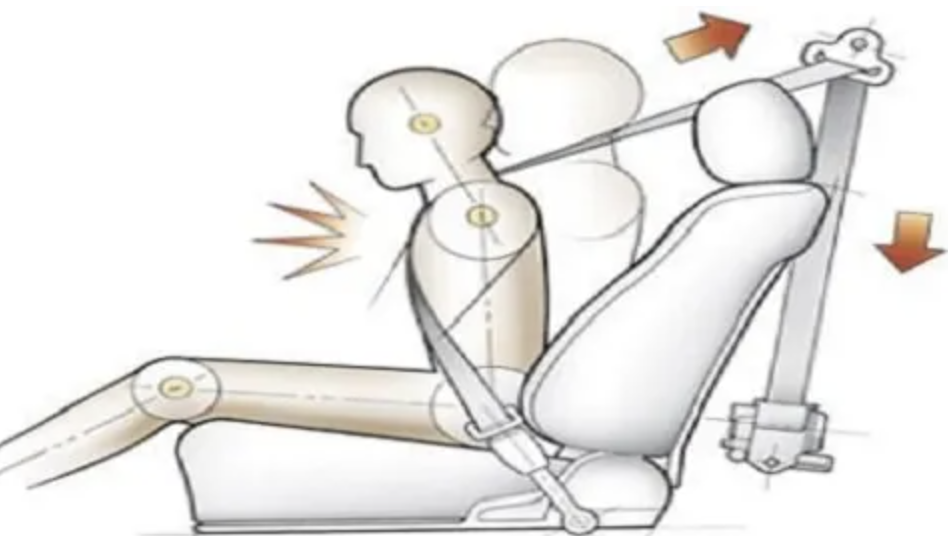
\includegraphics[width=.4\textwidth]{assets/c2b28cb9.png}
    \par}
\end{frame}

\begin{frame}{汽車上的應用Application to vehicles}
    \begin{itemize}
        \item 氣袋具有彈性 $\Rightarrow$ 增加撞擊時間 $\Rightarrow$ 減少碰撞期間的平均撞擊力。\\Air-bag is elastic $\Rightarrow$ Increase the time of impact  $\Rightarrow$ reduce average impact force during collision.
    \end{itemize}
    \bigskip
    {\par\centering
        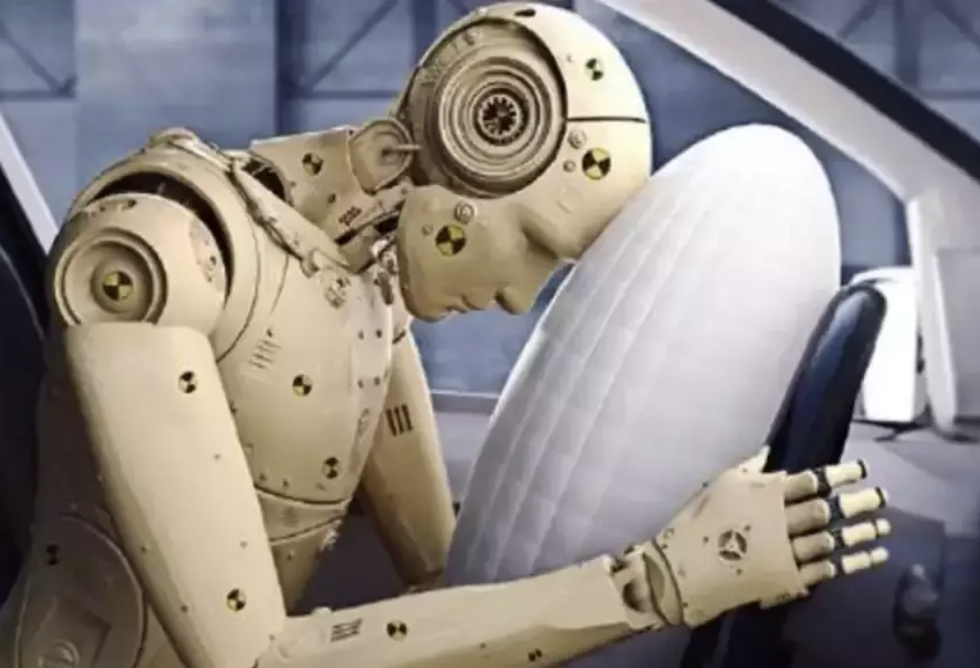
\includegraphics[width=.5\textwidth]{assets/5a24494a.png}
        \par}
\end{frame}

\begin{frame}{汽車上的應用Application to vehicles}
    \begin{itemize}
        \item 汽車泵把具有彈性 $\Rightarrow$ 增加撞擊時間 $\Rightarrow$ 減少碰撞期間的平均撞擊力。\\Car bumper is elastic $\Rightarrow$ Increase the time of impact  $\Rightarrow$ reduce average impact force during collision.
    \end{itemize}\bigskip
    {\par\centering
        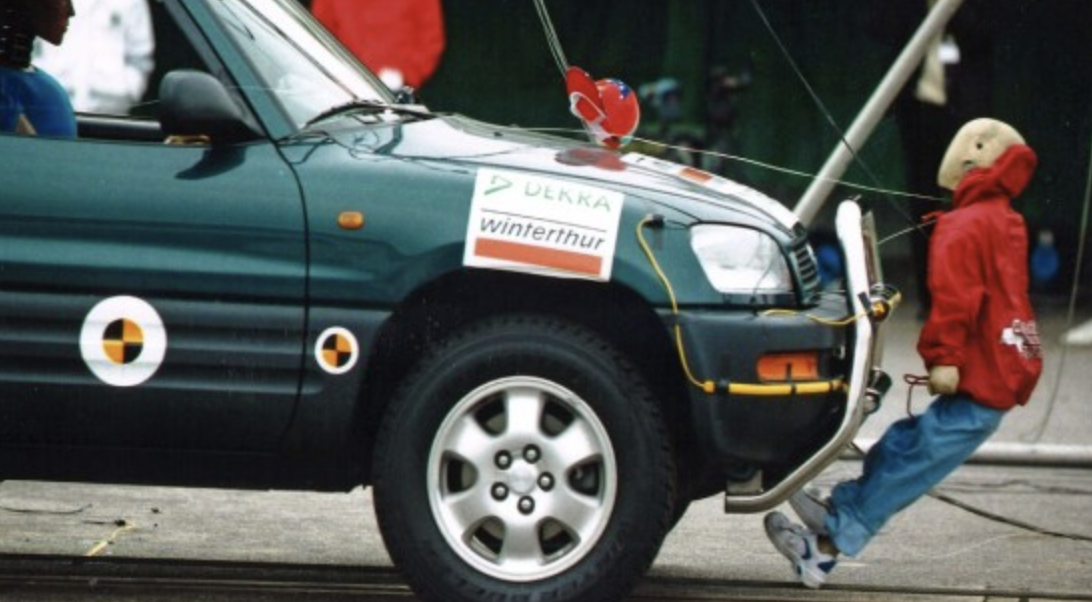
\includegraphics[width=.6\textwidth]{assets/b4012cdb.png}
        \par}
\end{frame}






















































\end{document}